% Requires in the preamble:
% \usepackage{amsmath,amssymb}
% \usepackage{tikz,pgfplots}
% \pgfplotsset{compat=1.18}

\chapter{Coordinate Geometry}
\label{app:coordinate-geometry}

Calculus draws many pictures: tangent lines, areas between curves, solids of
revolution, phase lines, parametric paths, and polar curves.  But a picture becomes
usable only when we can attach coordinates to it.

Coordinate geometry is the bridge.

\[
\text{geometry}
\quad\longleftrightarrow\quad
\text{algebra}.
\]

A line becomes an equation.  A circle becomes a distance condition.  A parabola
becomes a squared expression.  Shifting a graph becomes replacing \(x\) by
\(x-h\) or \(y\) by \(y-k\).

This appendix reviews the coordinate geometry used throughout the book.  The
goal is not to memorize many separate forms.  The goal is to recognize what an
equation is telling the picture to do.

\section{Lines}
\label{appsec:lines}

The first graph in calculus is often a line.  Constant velocity gives a line.  A
tangent approximation gives a line.  Newton's method follows a line.  The Mean
Value Theorem compares a tangent slope with a secant slope.

So lines deserve to be completely familiar.

\subsection{Slope}
\label{appsubsec:slope}

A nonvertical line has a constant steepness.  That steepness is its \emph{slope}.

If a line passes through two distinct points

\[
(x_1,y_1)
\qquad\text{and}\qquad
(x_2,y_2),
\]

with \(x_1\neq x_2\), then its slope is

\[
\boxed{
m=\frac{y_2-y_1}{x_2-x_1}.
}
\]

In words,

\[
\boxed{
\text{slope}=\frac{\text{change in }y}{\text{change in }x}
=
\frac{\text{rise}}{\text{run}}.
}
\]

\begin{figure}[h]
\centering
\begin{tikzpicture}
\begin{axis}[
    width=0.70\textwidth,
    height=0.43\textwidth,
    xmin=0, xmax=6,
    ymin=0, ymax=5,
    axis lines=left,
    xlabel={\(x\)},
    ylabel={\(y\)},
    xtick={1,5},
    ytick={1,4},
    grid=both,
    grid style={line width=.1pt, draw=gray!25},
]
\addplot[very thick, domain=0.6:5.5, samples=2] {0.75*x+0.25};
\addplot[only marks, mark=*] coordinates {(1,1) (5,4)};
\draw[dashed, thick] (axis cs:1,1) -- (axis cs:5,1);
\draw[dashed, thick] (axis cs:5,1) -- (axis cs:5,4);
\node[anchor=north] at (axis cs:3,1) {\(\Delta x=4\)};
\node[anchor=west] at (axis cs:5,2.5) {\(\Delta y=3\)};
\node[anchor=east] at (axis cs:1,1.15) {\((1,1)\)};
\node[anchor=west] at (axis cs:5,4) {\((5,4)\)};
\node[anchor=west] at (axis cs:2.4,3.2) {\(m=\dfrac34\)};
\end{axis}
\end{tikzpicture}
\caption{Slope measures vertical change per horizontal change.}
\label{fig:appendix-slope-rise-run}
\end{figure}

\paragraph{Example.}
Find the slope of the line through

\[
(1,1)
\qquad\text{and}\qquad
(5,4).
\]

The change in \(y\) is

\[
4-1=3.
\]

The change in \(x\) is

\[
5-1=4.
\]

Therefore

\[
\boxed{
m=\frac34.
}
\]

The line rises \(3\) units for every \(4\) units it moves to the right.

\paragraph{Example.}
Find the slope of the line through

\[
(2,5)
\qquad\text{and}\qquad
(6,-3).
\]

We compute

\[
m=\frac{-3-5}{6-2}=\frac{-8}{4}=-2.
\]

The negative sign means the line falls as \(x\) increases.

\begin{quote}
\textbf{Vertical lines.}
A vertical line has no slope, because its run is \(0\).  The slope formula would
require division by \(0\).

A vertical line has equation

\[
x=a.
\]

A horizontal line has slope \(0\) and equation

\[
y=b.
\]
\end{quote}

\subsection{Point-slope form}
\label{appsubsec:point-slope-form}

If a line has slope \(m\) and passes through the point

\[
(x_1,y_1),
\]

then every point \((x,y)\) on the line satisfies

\[
\frac{y-y_1}{x-x_1}=m
\]

when \(x\neq x_1\).  Multiplying by \(x-x_1\) gives the most useful form:

\[
\boxed{
y-y_1=m(x-x_1).
}
\]

This is called the \emph{point-slope form} of a line.

It is the same form used for tangent lines in calculus:

\[
y-f(a)=f'(a)(x-a).
\]

\paragraph{Example.}
Find an equation of the line through

\[
(2,-1)
\]

with slope

\[
m=\frac32.
\]

Use point-slope form:

\[
y-(-1)=\frac32(x-2).
\]

Thus

\[
\boxed{
y+1=\frac32(x-2).
}
\]

If we solve for \(y\),

\[
y+1=\frac32x-3,
\]

so

\[
\boxed{
y=\frac32x-4.
}
\]

\subsection{Slope-intercept form}
\label{appsubsec:slope-intercept-form}

If a line has slope \(m\) and crosses the \(y\)-axis at

\[
(0,b),
\]

then point-slope form gives

\[
y-b=m(x-0).
\]

So

\[
\boxed{
y=mx+b.
}
\]

This is the \emph{slope-intercept form}.  The number \(b\) is the
\emph{\(y\)-intercept}.

\paragraph{Example.}
The line

\[
y=-2x+5
\]

has slope

\[
m=-2
\]

and \(y\)-intercept

\[
b=5.
\]

So it crosses the \(y\)-axis at

\[
(0,5).
\]

It falls \(2\) units for every \(1\) unit it moves to the right.

\subsection{Line through two points}
\label{appsubsec:line-through-two-points}

To find a line through two points:

\[
\text{first find the slope, then use point-slope form.}
\]

\paragraph{Example.}
Find an equation of the line through

\[
(1,4)
\qquad\text{and}\qquad
(5,-2).
\]

First compute the slope:

\[
m=\frac{-2-4}{5-1}=\frac{-6}{4}=-\frac32.
\]

Use point-slope form with \((1,4)\):

\[
y-4=-\frac32(x-1).
\]

This is already a good equation.  If we want slope-intercept form,

\[
y-4=-\frac32x+\frac32,
\]

so

\[
\boxed{
y=-\frac32x+\frac{11}{2}.
}
\]

\subsection{General form}
\label{appsubsec:general-form-lines}

Every line can be written in the form

\[
\boxed{
Ax+By+C=0,
}
\]

where \(A\), \(B\), and \(C\) are constants, and \(A\) and \(B\) are not both \(0\).

If \(B\neq0\), then we can solve for \(y\):

\[
By=-Ax-C,
\]

so

\[
y=-\frac ABx-\frac CB.
\]

Therefore the slope is

\[
\boxed{
m=-\frac AB
}
\]

and the \(y\)-intercept is

\[
\boxed{
b=-\frac CB.
}
\]

If \(B=0\), the equation becomes

\[
Ax+C=0,
\]

so

\[
x=-\frac CA.
\]

That is a vertical line.

\paragraph{Example.}
Find the slope and intercepts of

\[
3x-5y=15.
\]

Solve for \(y\):

\[
-5y=15-3x.
\]

Thus

\[
y=\frac35x-3.
\]

So the slope is

\[
\boxed{\frac35}
\]

and the \(y\)-intercept is

\[
\boxed{(0,-3)}.
\]

To find the \(x\)-intercept, set \(y=0\):

\[
3x=15,
\]

so

\[
x=5.
\]

Thus the \(x\)-intercept is

\[
\boxed{(5,0)}.
\]

\begin{figure}[h]
\centering
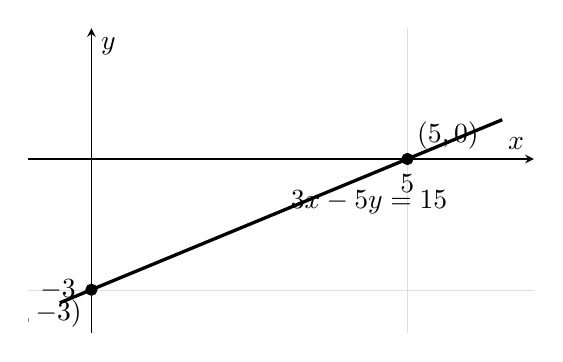
\begin{tikzpicture}
\begin{axis}[
    width=0.66\textwidth,
    height=0.45\textwidth,
    xmin=-1, xmax=7,
    ymin=-4, ymax=3,
    axis lines=middle,
    xlabel={\(x\)},
    ylabel={\(y\)},
    xtick={0,5},
    ytick={-3,0},
    grid=both,
    grid style={line width=.1pt, draw=gray!25},
]
\addplot[very thick, domain=-0.5:6.5, samples=2] {(3/5)*x-3};
\addplot[only marks, mark=*] coordinates {(0,-3) (5,0)};
\node[anchor=north east] at (axis cs:0,-3) {\((0,-3)\)};
\node[anchor=south west] at (axis cs:5,0) {\((5,0)\)};
\node[anchor=west] at (axis cs:3.0,-1.0) {\(3x-5y=15\)};
\end{axis}
\end{tikzpicture}
\caption{The intercepts are often the quickest way to sketch a line in general form.}
\label{fig:appendix-line-intercepts}
\end{figure}

\subsection{Parallel and perpendicular lines}
\label{appsubsec:parallel-perpendicular-lines}

Slope detects parallel and perpendicular lines.

\begin{quote}
\textbf{Parallel lines.}
Two nonvertical lines are parallel exactly when they have the same slope.
\end{quote}

\begin{quote}
\textbf{Perpendicular lines.}
Two nonvertical lines with slopes \(m_1\) and \(m_2\) are perpendicular exactly when

\[
\boxed{
m_1m_2=-1.
}
\]

Equivalently,

\[
m_2=-\frac1{m_1}.
\]
\end{quote}

A vertical line is perpendicular to a horizontal line.

\paragraph{Example.}
Find the line through

\[
(-1,2)
\]

parallel to

\[
2x-3y=6.
\]

First solve the given line for \(y\):

\[
-3y=6-2x,
\]

so

\[
y=\frac23x-2.
\]

The slope is

\[
m=\frac23.
\]

A parallel line has the same slope.  Using point-slope form,

\[
y-2=\frac23(x+1).
\]

Thus

\[
\boxed{
y=\frac23x+\frac83.
}
\]

\paragraph{Example.}
Find the line through

\[
(4,-1)
\]

perpendicular to

\[
y=-4x+7.
\]

The given line has slope

\[
-4.
\]

A perpendicular line has slope

\[
\frac14,
\]

because

\[
(-4)\left(\frac14\right)=-1.
\]

Thus

\[
y+1=\frac14(x-4).
\]

So

\[
\boxed{
y=\frac14x-2.
}
\]

\section{Circles}
\label{appsec:circles}

A circle is a distance condition.

Choose a center

\[
(h,k)
\]

and a radius \(r>0\).  A point \((x,y)\) lies on the circle if its distance from
\((h,k)\) is exactly \(r\).

That sentence becomes an equation.

\subsection{Equation of a circle}
\label{appsubsec:equation-circle}

The distance from \((x,y)\) to \((h,k)\) is

\[
\sqrt{(x-h)^2+(y-k)^2}.
\]

So the circle condition is

\[
\sqrt{(x-h)^2+(y-k)^2}=r.
\]

Squaring both sides gives

\[
\boxed{
(x-h)^2+(y-k)^2=r^2.
}
\]

This is the standard equation of a circle with center \((h,k)\) and radius \(r\).

If the center is the origin, the equation becomes

\[
\boxed{
x^2+y^2=r^2.
}
\]

\paragraph{Example.}
Find an equation of the circle with center

\[
(2,-3)
\]

and radius

\[
5.
\]

Use the standard form:

\[
(x-2)^2+(y-(-3))^2=5^2.
\]

Thus

\[
\boxed{
(x-2)^2+(y+3)^2=25.
}
\]

\begin{figure}[h]
\centering
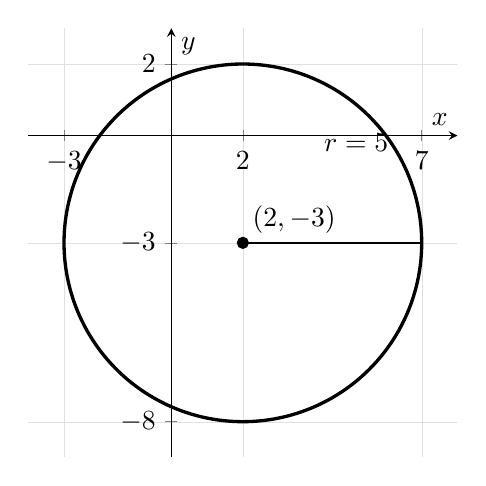
\begin{tikzpicture}
\begin{axis}[
    width=0.58\textwidth,
    height=0.58\textwidth,
    xmin=-4, xmax=8,
    ymin=-9, ymax=3,
    axis lines=middle,
    xlabel={\(x\)},
    ylabel={\(y\)},
    xtick={-3,0,2,7},
    ytick={-8,-3,0,2},
    grid=both,
    grid style={line width=.1pt, draw=gray!25},
    axis equal image,
]
\addplot[very thick, domain=0:360, samples=200] ({2+5*cos(x)}, {-3+5*sin(x)});
\addplot[only marks, mark=*] coordinates {(2,-3)};
\node[anchor=south west] at (axis cs:2,-3) {\((2,-3)\)};
\node[anchor=west] at (axis cs:4.0,-0.2) {\(r=5\)};
\draw[thick] (axis cs:2,-3) -- (axis cs:7,-3);
\end{axis}
\end{tikzpicture}
\caption{The circle \((x-2)^2+(y+3)^2=25\) has center \((2,-3)\) and radius \(5\).}
\label{fig:appendix-circle-center-radius}
\end{figure}

\subsection{Completing the square}
\label{appsubsec:circle-completing-square}

A circle is not always written in standard form.  Completing the square reveals the
center and radius.

\paragraph{Example.}
Show that

\[
x^2+y^2-6x+4y-12=0
\]

is a circle, and find its center and radius.

Group the \(x\)-terms and \(y\)-terms:

\[
x^2-6x+y^2+4y=12.
\]

Complete the square in each variable:

\[
x^2-6x=(x-3)^2-9,
\]

and

\[
y^2+4y=(y+2)^2-4.
\]

Substitute:

\[
(x-3)^2-9+(y+2)^2-4=12.
\]

Thus

\[
(x-3)^2+(y+2)^2=25.
\]

So the center is

\[
\boxed{(3,-2)}
\]

and the radius is

\[
\boxed{5}.
\]

\subsection{Disks and circle inequalities}
\label{appsubsec:circle-inequalities}

A circle is the boundary.  A disk is the filled-in region.

The equation

\[
(x-h)^2+(y-k)^2=r^2
\]

means distance exactly \(r\) from \((h,k)\).

The inequality

\[
(x-h)^2+(y-k)^2<r^2
\]

means distance less than \(r\).  This is the inside of the circle, without the boundary.

The inequality

\[
(x-h)^2+(y-k)^2\le r^2
\]

means the inside together with the boundary.

\begin{center}
\renewcommand{\arraystretch}{1.5}
\begin{tabular}{c|c}
\textbf{condition} & \textbf{region} \\ \hline
\((x-h)^2+(y-k)^2=r^2\) & circle \\
\((x-h)^2+(y-k)^2<r^2\) & inside, boundary excluded \\
\((x-h)^2+(y-k)^2\le r^2\) & inside, boundary included \\
\((x-h)^2+(y-k)^2>r^2\) & outside, boundary excluded
\end{tabular}
\end{center}

\paragraph{Example.}
Describe the region

\[
(x-1)^2+(y+3)^2\le 9.
\]

The center is

\[
(1,-3),
\]

and the radius is

\[
3.
\]

Because the inequality is \(\le\), the region is the closed disk: all points whose
distance from \((1,-3)\) is at most \(3\).

\section{Parabolas, ellipses, and hyperbolas}
\label{appsec:conics}

Lines and circles are not the only curves that appear in calculus.  Parabolas are
the basic graphs of quadratic functions.  Ellipses appear in planetary motion and
optimization.  Hyperbolas appear in reciprocal functions, asymptotes, and polar
coordinates.

These curves are called \emph{conic sections}, or simply \emph{conics}, because
they can be obtained by slicing a cone with a plane.  For our purposes, the most
important skill is algebraic recognition.

\[
\text{Which squared terms appear?}
\qquad
\text{What are their signs?}
\qquad
\text{Can we complete the square?}
\]

\subsection{Parabolas}
\label{appsubsec:parabolas}

A vertical parabola has vertex form

\[
\boxed{
y=a(x-h)^2+k.
}
\]

Its vertex is

\[
(h,k).
\]

If \(a>0\), it opens upward.  If \(a<0\), it opens downward.

A horizontal parabola has form

\[
\boxed{
x=a(y-k)^2+h.
}
\]

If \(a>0\), it opens to the right.  If \(a<0\), it opens to the left.

\paragraph{Example.}
Describe the graph of

\[
y=2(x-1)^2-3.
\]

The vertex is

\[
(1,-3).
\]

Since \(a=2>0\), the parabola opens upward.  Compared with

\[
y=x^2,
\]

it is shifted right \(1\), shifted down \(3\), and vertically stretched by a factor of \(2\).

\begin{figure}[h]
\centering
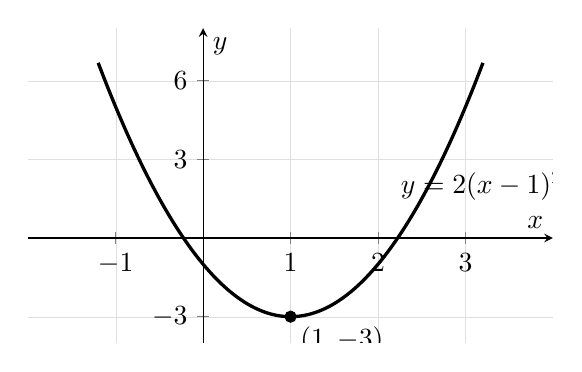
\begin{tikzpicture}
\begin{axis}[
    width=0.68\textwidth,
    height=0.46\textwidth,
    xmin=-2, xmax=4,
    ymin=-4, ymax=8,
    axis lines=middle,
    xlabel={\(x\)},
    ylabel={\(y\)},
    xtick={-1,0,1,2,3},
    ytick={-3,0,3,6},
    grid=both,
    grid style={line width=.1pt, draw=gray!25},
]
\addplot[very thick, domain=-1.2:3.2, samples=150] {2*(x-1)^2-3};
\addplot[only marks, mark=*] coordinates {(1,-3)};
\node[anchor=north west] at (axis cs:1,-3) {\((1,-3)\)};
\node[anchor=west] at (axis cs:2.15,2.0) {\(y=2(x-1)^2-3\)};
\end{axis}
\end{tikzpicture}
\caption{Vertex form shows the shift and stretch immediately.}
\label{fig:appendix-parabola-vertex-form}
\end{figure}

\paragraph{Example.}
Rewrite

\[
y=x^2-6x+5
\]

in vertex form.

Complete the square:

\[
x^2-6x=(x-3)^2-9.
\]

Therefore

\[
y=(x-3)^2-9+5.
\]

So

\[
\boxed{
y=(x-3)^2-4.
}
\]

The vertex is

\[
\boxed{(3,-4)}.
\]

\subsection{Focus and directrix form}
\label{appsubsec:focus-directrix-parabola}

A parabola can also be defined as a distance condition: points equidistant from a
fixed point and a fixed line.

For a vertical parabola with vertex \((h,k)\),

\[
\boxed{
(x-h)^2=4p(y-k)
}
\]

has focus

\[
(h,k+p)
\]

and directrix

\[
y=k-p.
\]

The number \(p\) gives the signed distance from the vertex to the focus.  If
\(p>0\), the parabola opens upward.  If \(p<0\), it opens downward.

For a horizontal parabola,

\[
\boxed{
(y-k)^2=4p(x-h)
}
\]

has focus

\[
(h+p,k)
\]

and directrix

\[
x=h-p.
\]

\paragraph{Example.}
Find the focus and directrix of

\[
x^2=8y.
\]

Compare with

\[
x^2=4py.
\]

So

\[
4p=8,
\qquad
p=2.
\]

The vertex is the origin.  Therefore the focus is

\[
\boxed{(0,2)}
\]

and the directrix is

\[
\boxed{y=-2}.
\]

\subsection{Ellipses}
\label{appsubsec:ellipses}

An ellipse is an oval.  Its standard equation is

\[
\boxed{
\frac{(x-h)^2}{a^2}+\frac{(y-k)^2}{b^2}=1.
}
\]

The center is

\[
(h,k).
\]

The horizontal semi-axis length is \(a\).  The vertical semi-axis length is \(b\).
The full width is \(2a\), and the full height is \(2b\).

\begin{figure}[h]
\centering
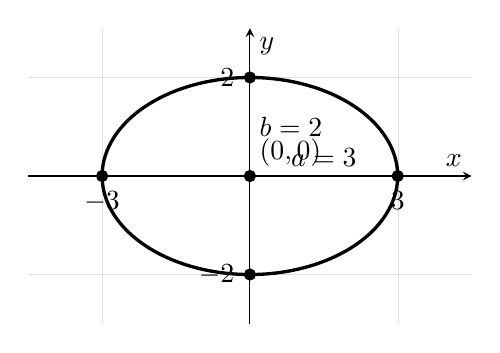
\begin{tikzpicture}
\begin{axis}[
    width=0.68\textwidth,
    height=0.44\textwidth,
    xmin=-4.5, xmax=4.5,
    ymin=-3, ymax=3,
    axis lines=middle,
    xlabel={\(x\)},
    ylabel={\(y\)},
    xtick={-3,0,3},
    ytick={-2,0,2},
    grid=both,
    grid style={line width=.1pt, draw=gray!25},
    axis equal image,
]
\addplot[very thick, domain=0:360, samples=250] ({3*cos(x)}, {2*sin(x)});
\addplot[only marks, mark=*] coordinates {(0,0) (3,0) (-3,0) (0,2) (0,-2)};
\node[anchor=south west] at (axis cs:0,0) {\((0,0)\)};
\node[anchor=south] at (axis cs:1.5,0) {\(a=3\)};
\node[anchor=west] at (axis cs:0,1) {\(b=2\)};
\end{axis}
\end{tikzpicture}
\caption{The ellipse \(\frac{x^2}{9}+\frac{y^2}{4}=1\) has semi-axis lengths \(3\) and \(2\).}
\label{fig:appendix-ellipse-standard}
\end{figure}

\paragraph{Example.}
Describe the ellipse

\[
\frac{(x+2)^2}{16}+\frac{(y-1)^2}{9}=1.
\]

The center is

\[
(-2,1).
\]

The horizontal semi-axis length is

\[
4,
\]

because \(16=4^2\).  The vertical semi-axis length is

\[
3,
\]

because \(9=3^2\).

So the ellipse has width \(8\) and height \(6\).

\subsection{Hyperbolas}
\label{appsubsec:hyperbolas}

A hyperbola has two branches and two asymptotes.

A horizontal hyperbola has standard form

\[
\boxed{
\frac{(x-h)^2}{a^2}-\frac{(y-k)^2}{b^2}=1.
}
\]

It opens left and right.  Its center is \((h,k)\).  Its vertices are

\[
(h-a,k)
\qquad\text{and}\qquad
(h+a,k).
\]

Its asymptotes are

\[
\boxed{
y-k=\pm\frac ba(x-h).
}
\]

A vertical hyperbola has standard form

\[
\boxed{
\frac{(y-k)^2}{a^2}-\frac{(x-h)^2}{b^2}=1.
}
\]

It opens up and down.  Its vertices are

\[
(h,k-a)
\qquad\text{and}\qquad
(h,k+a).
\]

Its asymptotes are

\[
\boxed{
y-k=\pm\frac ab(x-h).
}
\]

\paragraph{Example.}
Describe

\[
\frac{x^2}{9}-\frac{y^2}{4}=1.
\]

This is a horizontal hyperbola centered at the origin.  Here

\[
a=3,
\qquad
b=2.
\]

The vertices are

\[
(-3,0)
\qquad\text{and}\qquad
(3,0).
\]

The asymptotes are

\[
\boxed{
y=\pm\frac23x.
}
\]

\begin{figure}[h]
\centering
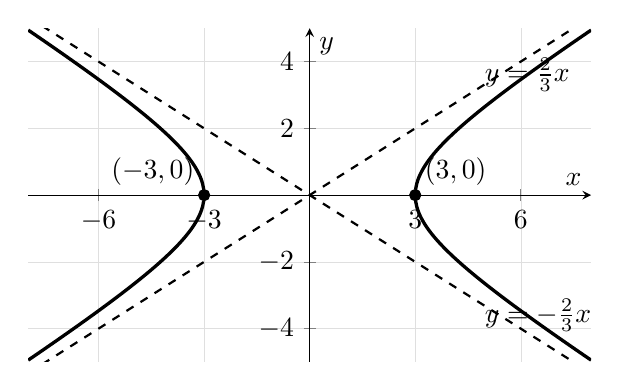
\begin{tikzpicture}
\begin{axis}[
    width=0.72\textwidth,
    height=0.48\textwidth,
    xmin=-8, xmax=8,
    ymin=-5, ymax=5,
    axis lines=middle,
    xlabel={\(x\)},
    ylabel={\(y\)},
    xtick={-6,-3,0,3,6},
    ytick={-4,-2,0,2,4},
    grid=both,
    grid style={line width=.1pt, draw=gray!25},
]
\addplot[very thick, domain=3.01:8, samples=150] {(2/3)*sqrt(x^2-9)};
\addplot[very thick, domain=3.01:8, samples=150] {-(2/3)*sqrt(x^2-9)};
\addplot[very thick, domain=-8:-3.01, samples=150] {(2/3)*sqrt(x^2-9)};
\addplot[very thick, domain=-8:-3.01, samples=150] {-(2/3)*sqrt(x^2-9)};
\addplot[thick, dashed, domain=-8:8, samples=2] {(2/3)*x};
\addplot[thick, dashed, domain=-8:8, samples=2] {-(2/3)*x};
\addplot[only marks, mark=*] coordinates {(-3,0) (3,0)};
\node[anchor=south west] at (axis cs:3,0) {\((3,0)\)};
\node[anchor=south east] at (axis cs:-3,0) {\((-3,0)\)};
\node[anchor=west] at (axis cs:4.7,3.6) {\(y=\frac23x\)};
\node[anchor=west] at (axis cs:4.7,-3.6) {\(y=-\frac23x\)};
\end{axis}
\end{tikzpicture}
\caption{A hyperbola approaches its asymptotes but does not cross them far from the center.}
\label{fig:appendix-hyperbola-asymptotes}
\end{figure}

\paragraph{Example: completing the square for a hyperbola.}
Put

\[
9y^2-18y-4x^2-4x=28
\]

in standard form.

Group terms:

\[
9(y^2-2y)-4(x^2+x)=28.
\]

Complete the square inside each group:

\[
y^2-2y=(y-1)^2-1,
\]

and

\[
x^2+x=\left(x+\frac12\right)^2-\frac14.
\]

Substitute:

\[
9\bigl((y-1)^2-1\bigr)
-
4\left(\left(x+\frac12\right)^2-\frac14\right)
=
28.
\]

Expand the constants:

\[
9(y-1)^2-9
-
4\left(x+\frac12\right)^2
+1
=
28.
\]

So

\[
9(y-1)^2-4\left(x+\frac12\right)^2=36.
\]

Divide by \(36\):

\[
\boxed{
\frac{(y-1)^2}{4}
-
\frac{\left(x+\frac12\right)^2}{9}
=
1.
}
\]

This is a vertical hyperbola with center

\[
\boxed{
\left(-\frac12,1\right).
}
\]

Since \(a=2\) and \(b=3\), the vertices are

\[
\left(-\frac12,1-2\right)
\qquad\text{and}\qquad
\left(-\frac12,1+2\right).
\]

Thus the vertices are

\[
\boxed{
\left(-\frac12,-1\right)
\quad\text{and}\quad
\left(-\frac12,3\right).
}
\]

The asymptotes are

\[
\boxed{
y-1=\pm\frac23\left(x+\frac12\right).
}
\]

\subsection{Recognizing conics quickly}
\label{appsubsec:recognizing-conics}

When no \(xy\)-term appears, the squared terms give a quick first test.

\begin{center}
\renewcommand{\arraystretch}{1.6}
\begin{tabular}{c|c|c}
\textbf{equation pattern} & \textbf{shape} & \textbf{main clue} \\ \hline
one squared variable & parabola & only \(x^2\) or only \(y^2\) \\
\(x^2\) and \(y^2\), same sign & circle or ellipse & both squared terms add \\
\(x^2\) and \(y^2\), opposite signs & hyperbola & squared terms subtract
\end{tabular}
\end{center}

A circle is the special ellipse in which the two squared terms have the same
coefficient after completing the square.

\paragraph{Example.}
Identify the type of conic:

\[
4x^2+y^2-16x+6y+21=0.
\]

Both squared terms appear and have the same sign, so the graph is an ellipse or
possibly a circle.  Complete the square:

\[
4(x^2-4x)+(y^2+6y)=-21.
\]

Now

\[
x^2-4x=(x-2)^2-4,
\]

and

\[
y^2+6y=(y+3)^2-9.
\]

So

\[
4\bigl((x-2)^2-4\bigr)+(y+3)^2-9=-21.
\]

Thus

\[
4(x-2)^2-16+(y+3)^2-9=-21.
\]

So

\[
4(x-2)^2+(y+3)^2=4.
\]

Divide by \(4\):

\[
\boxed{
(x-2)^2+\frac{(y+3)^2}{4}=1.
}
\]

This is an ellipse centered at

\[
(2,-3).
\]

\section{Distance and midpoint formulas}
\label{appsec:distance-midpoint}

Distance turns coordinate geometry into measurement.  The distance formula is just
the Pythagorean Theorem written with coordinates.

\subsection{Distance between two points}
\label{appsubsec:distance-between-points}

Let

\[
P_1=(x_1,y_1)
\qquad\text{and}\qquad
P_2=(x_2,y_2).
\]

The horizontal change from \(P_1\) to \(P_2\) is

\[
x_2-x_1.
\]

The vertical change is

\[
y_2-y_1.
\]

These are the legs of a right triangle.  Therefore the distance between the points is

\[
\boxed{
d(P_1,P_2)
=
\sqrt{(x_2-x_1)^2+(y_2-y_1)^2}.
}
\]

\begin{figure}[h]
\centering
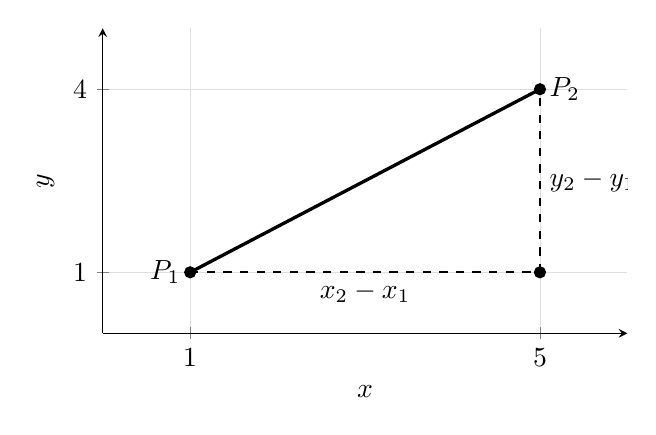
\begin{tikzpicture}
\begin{axis}[
    width=0.68\textwidth,
    height=0.45\textwidth,
    xmin=0, xmax=6,
    ymin=0, ymax=5,
    axis lines=left,
    xlabel={\(x\)},
    ylabel={\(y\)},
    xtick={1,5},
    ytick={1,4},
    grid=both,
    grid style={line width=.1pt, draw=gray!25},
]
\addplot[only marks, mark=*] coordinates {(1,1) (5,4) (5,1)};
\draw[very thick] (axis cs:1,1) -- (axis cs:5,4);
\draw[dashed, thick] (axis cs:1,1) -- (axis cs:5,1);
\draw[dashed, thick] (axis cs:5,1) -- (axis cs:5,4);
\node[anchor=east] at (axis cs:1,1) {\(P_1\)};
\node[anchor=west] at (axis cs:5,4) {\(P_2\)};
\node[anchor=north] at (axis cs:3,1) {\(x_2-x_1\)};
\node[anchor=west] at (axis cs:5,2.5) {\(y_2-y_1\)};
\end{axis}
\end{tikzpicture}
\caption{The distance formula is the Pythagorean Theorem.}
\label{fig:appendix-distance-formula}
\end{figure}

\paragraph{Example.}
Find the distance between

\[
(-2,3)
\qquad\text{and}\qquad
(4,-5).
\]

Use the formula:

\[
d=\sqrt{(4-(-2))^2+(-5-3)^2}.
\]

So

\[
d=\sqrt{6^2+(-8)^2}
=
\sqrt{36+64}
=
\sqrt{100}
=
\boxed{10}.
\]

\subsection{Midpoint of a segment}
\label{appsubsec:midpoint}

The midpoint is halfway in the \(x\)-direction and halfway in the \(y\)-direction.

If

\[
P_1=(x_1,y_1)
\qquad\text{and}\qquad
P_2=(x_2,y_2),
\]

then the midpoint is

\[
\boxed{
M=
\left(
\frac{x_1+x_2}{2},
\frac{y_1+y_2}{2}
\right).
}
\]

\paragraph{Example.}
Find the midpoint of the segment joining

\[
(-2,3)
\qquad\text{and}\qquad
(4,-5).
\]

Average the \(x\)-coordinates:

\[
\frac{-2+4}{2}=1.
\]

Average the \(y\)-coordinates:

\[
\frac{3+(-5)}{2}=-1.
\]

So the midpoint is

\[
\boxed{
(1,-1).
}
\]

\subsection{A locus example: perpendicular bisectors}
\label{appsubsec:locus-perpendicular-bisector}

A \emph{locus} is a set of points satisfying a condition.

For example, the perpendicular bisector of a segment is the set of all points
equidistant from the segment's endpoints.

\paragraph{Example.}
Find the set of points \((x,y)\) equidistant from

\[
A=(0,0)
\]

and

\[
B=(4,2).
\]

Equidistant means

\[
d((x,y),A)=d((x,y),B).
\]

Using squared distances avoids square roots:

\[
x^2+y^2=(x-4)^2+(y-2)^2.
\]

Expand the right side:

\[
x^2+y^2=x^2-8x+16+y^2-4y+4.
\]

Cancel \(x^2+y^2\) from both sides:

\[
0=-8x-4y+20.
\]

Thus

\[
8x+4y=20.
\]

Divide by \(4\):

\[
\boxed{
2x+y=5.
}
\]

This line is the perpendicular bisector of the segment from \(A\) to \(B\).

\begin{quote}
\textbf{Why squared distances are allowed.}
Distance is nonnegative.  If two distances are equal, then their squares are equal.
Conversely, if two nonnegative distances have equal squares, then the distances are
equal.
\end{quote}

\section{Scaling and shifting graphs}
\label{appsec:scaling-shifting-graphs}

Many graphs in calculus come from simpler graphs by shifting, stretching, and
reflecting.

If we understand the parent graph, transformations let us sketch the new graph
quickly.  More importantly, they tell us how the formula changes the geometry.

\subsection{Vertical and horizontal shifts}
\label{appsubsec:vertical-horizontal-shifts}

Let \(y=f(x)\).

The graph of

\[
y=f(x)+k
\]

is the graph of \(y=f(x)\) shifted vertically by \(k\).

If \(k>0\), the graph moves up.  If \(k<0\), it moves down.

The graph of

\[
y=f(x-h)
\]

is the graph of \(y=f(x)\) shifted horizontally by \(h\).

If \(h>0\), the graph moves right.  If \(h<0\), it moves left.

\begin{center}
\renewcommand{\arraystretch}{1.6}
\begin{tabular}{c|c}
\textbf{new function} & \textbf{effect on graph of \(y=f(x)\)} \\ \hline
\(f(x)+k\) & shift up by \(k\) if \(k>0\), down if \(k<0\) \\
\(f(x-h)\) & shift right by \(h\) if \(h>0\), left if \(h<0\)
\end{tabular}
\end{center}

\paragraph{Example.}
Start with

\[
f(x)=x^2.
\]

Then

\[
g(x)=(x-3)^2-1
\]

is the graph of \(x^2\) shifted right \(3\) and down \(1\).  Its vertex is

\[
(3,-1).
\]

\begin{figure}[h]
\centering
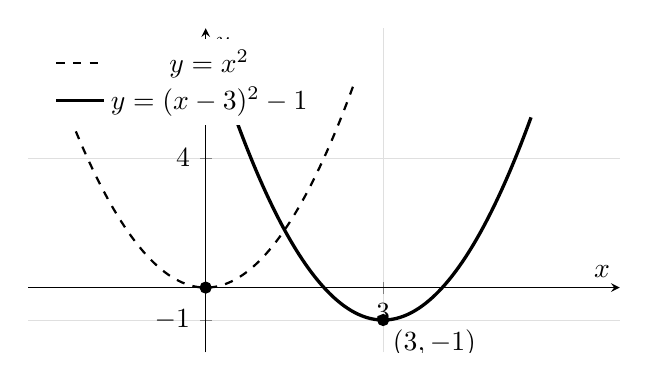
\begin{tikzpicture}
\begin{axis}[
    width=0.75\textwidth,
    height=0.47\textwidth,
    xmin=-3, xmax=7,
    ymin=-2, ymax=8,
    axis lines=middle,
    xlabel={\(x\)},
    ylabel={\(y\)},
    xtick={0,3},
    ytick={-1,0,4},
    grid=both,
    grid style={line width=.1pt, draw=gray!25},
    legend style={draw=none, at={(0.03,0.97)}, anchor=north west}
]
\addplot[thick, dashed, domain=-2.5:2.5, samples=120] {x^2};
\addlegendentry{\(y=x^2\)}
\addplot[very thick, domain=0.5:5.5, samples=120] {(x-3)^2-1};
\addlegendentry{\(y=(x-3)^2-1\)}
\addplot[only marks, mark=*] coordinates {(0,0) (3,-1)};
\node[anchor=north west] at (axis cs:3,-1) {\((3,-1)\)};
\end{axis}
\end{tikzpicture}
\caption{Replacing \(x\) by \(x-3\) shifts right \(3\); subtracting \(1\) shifts down \(1\).}
\label{fig:appendix-parabola-shift}
\end{figure}

\subsection{Vertical scaling and reflection}
\label{appsubsec:vertical-scaling-reflection}

The graph of

\[
y=af(x)
\]

is a vertical scaling of the graph of \(y=f(x)\).

If

\[
|a|>1,
\]

the graph stretches vertically.

If

\[
0<|a|<1,
\]

the graph compresses vertically.

If

\[
a<0,
\]

the graph is also reflected across the \(x\)-axis.

\paragraph{Example.}
Start with

\[
f(x)=\sqrt{x}.
\]

Then

\[
g(x)=-2\sqrt{x}
\]

is reflected across the \(x\)-axis and stretched vertically by \(2\).  Its domain is still

\[
[0,\infty),
\]

but its range is

\[
(-\infty,0].
\]

\subsection{Horizontal scaling and reflection}
\label{appsubsec:horizontal-scaling-reflection}

The graph of

\[
y=f(cx)
\]

is a horizontal scaling of the graph of \(y=f(x)\).

If

\[
|c|>1,
\]

the graph compresses horizontally by a factor of \(|c|\).

If

\[
0<|c|<1,
\]

the graph stretches horizontally by a factor of \(1/|c|\).

If

\[
c<0,
\]

the graph is also reflected across the \(y\)-axis.

This direction can feel backwards.  The reason is that the input is being changed
before \(f\) acts.

For example,

\[
f(2x)
\]

reaches the old input \(1\) when

\[
2x=1,
\]

so

\[
x=\frac12.
\]

Everything happens in half the horizontal distance.  The graph is compressed.

\begin{center}
\renewcommand{\arraystretch}{1.6}
\begin{tabular}{c|c}
\textbf{new function} & \textbf{effect on graph of \(y=f(x)\)} \\ \hline
\(af(x)\), \(a>1\) & vertical stretch by \(a\) \\
\(af(x)\), \(0<a<1\) & vertical compression by \(a\) \\
\(-f(x)\) & reflection across the \(x\)-axis \\
\(f(cx)\), \(c>1\) & horizontal compression by \(c\) \\
\(f(cx)\), \(0<c<1\) & horizontal stretch by \(1/c\) \\
\(f(-x)\) & reflection across the \(y\)-axis
\end{tabular}
\end{center}

\paragraph{Example.}
Compare

\[
y=\sin x
\]

and

\[
y=\sin(2x).
\]

The graph of \(\sin(2x)\) completes a full oscillation when

\[
2x=2\pi,
\]

so

\[
x=\pi.
\]

Thus its period is

\[
\pi,
\]

half the period of \(\sin x\).  The graph is horizontally compressed by \(2\).

\subsection{Transformations and domains}
\label{appsubsec:transformations-domains}

Transformations also affect domains and ranges.

\paragraph{Example.}
Find the domain and range of

\[
g(x)=\sqrt{x-2}+1.
\]

The square root requires

\[
x-2\ge0.
\]

So

\[
x\ge2.
\]

Thus the domain is

\[
\boxed{[2,\infty)}.
\]

Since

\[
\sqrt{x-2}\ge0,
\]

we have

\[
\sqrt{x-2}+1\ge1.
\]

Thus the range is

\[
\boxed{[1,\infty)}.
\]

The graph of \(y=\sqrt{x}\) has been shifted right \(2\) and up \(1\).

\begin{figure}[h]
\centering
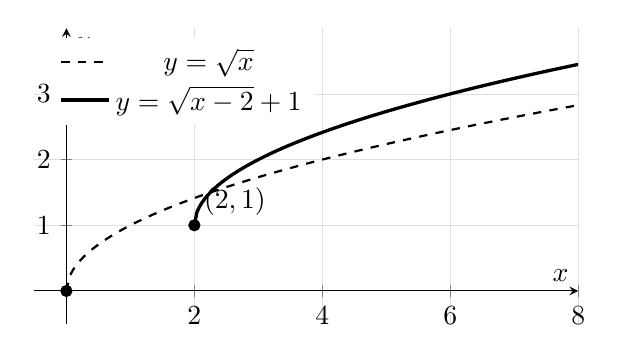
\begin{tikzpicture}
\begin{axis}[
    width=0.70\textwidth,
    height=0.44\textwidth,
    xmin=-0.5, xmax=8,
    ymin=-0.5, ymax=4,
    axis lines=middle,
    xlabel={\(x\)},
    ylabel={\(y\)},
    xtick={0,2,4,6,8},
    ytick={0,1,2,3},
    grid=both,
    grid style={line width=.1pt, draw=gray!25},
    legend style={draw=none, at={(0.03,0.97)}, anchor=north west}
]
\addplot[thick, dashed, domain=0:8, samples=150] {sqrt(x)};
\addlegendentry{\(y=\sqrt{x}\)}
\addplot[very thick, domain=2:8, samples=150] {sqrt(x-2)+1};
\addlegendentry{\(y=\sqrt{x-2}+1\)}
\addplot[only marks, mark=*] coordinates {(0,0) (2,1)};
\node[anchor=south west] at (axis cs:2,1) {\((2,1)\)};
\end{axis}
\end{tikzpicture}
\caption{The starting point of the square-root graph moves from \((0,0)\) to \((2,1)\).}
\label{fig:appendix-sqrt-shift}
\end{figure}

\subsection{Transforming equations}
\label{appsubsec:transforming-equations}

Transformations are not limited to functions.  They also apply to equations.

For example, the unit circle

\[
x^2+y^2=1
\]

becomes an ellipse if we stretch horizontally by \(3\) and vertically by \(2\).

A point on the stretched curve has the form

\[
x=3u,
\qquad
y=2v,
\]

where

\[
u^2+v^2=1.
\]

So

\[
u=\frac{x}{3},
\qquad
v=\frac{y}{2}.
\]

Substitute into the unit circle equation:

\[
\left(\frac{x}{3}\right)^2+\left(\frac{y}{2}\right)^2=1.
\]

Thus the stretched curve is

\[
\boxed{
\frac{x^2}{9}+\frac{y^2}{4}=1.
}
\]

If we then shift the ellipse up by \(1\), replace \(y\) by \(y-1\):

\[
\boxed{
\frac{x^2}{9}+\frac{(y-1)^2}{4}=1.
}
\]

This is an ellipse centered at

\[
(0,1)
\]

with horizontal semi-axis \(3\) and vertical semi-axis \(2\).

\begin{quote}
\textbf{Transformation warning.}
For graph transformations, the input changes in the opposite-looking direction.
The expression \(x-h\) shifts right by \(h\), not left.

A reliable check is to track a familiar point.  If the old graph starts at \((0,0)\),
then \(y=\sqrt{x-2}+1\) starts at \((2,1)\).
\end{quote}

\section{Practice problems}
\label{appsec:coordinate-geometry-practice}

\subsection*{Lines}

\begin{enumerate}
\item Find the slope of the line through \((2,3)\) and \((8,6)\).

\item Find the slope of the line through \((-1,4)\) and \((5,-8)\).

\item Find an equation of the line through \((3,-2)\) with slope \(4\).

\item Find an equation of the line through \((1,5)\) and \((4,-1)\).

\item Find the slope and \(y\)-intercept of
\[
2x+3y=12.
\]

\item Find an equation of the line through \((2,1)\) parallel to
\[
y=-3x+4.
\]

\item Find an equation of the line through \((-2,5)\) perpendicular to
\[
y=\frac12x-1.
\]

\item Find the \(x\)- and \(y\)-intercepts of
\[
4x-5y=20.
\]
\end{enumerate}

\subsection*{Circles}

\begin{enumerate}
\item Find an equation of the circle with center \((-1,4)\) and radius \(6\).

\item Find the center and radius of
\[
(x-3)^2+(y+2)^2=49.
\]

\item Put the equation
\[
x^2+y^2+8x-10y+16=0
\]
in standard circle form.

\item Describe the region
\[
(x+1)^2+(y-2)^2<16.
\]

\item Find the intersection points of
\[
x^2+y^2=25
\]
and
\[
y=3.
\]
\end{enumerate}

\subsection*{Parabolas, ellipses, and hyperbolas}

\begin{enumerate}
\item Rewrite
\[
y=x^2+4x-1
\]
in vertex form.

\item Find the vertex and opening direction of
\[
y=-3(x-2)^2+5.
\]

\item Find the focus and directrix of
\[
x^2=12y.
\]

\item Describe the ellipse
\[
\frac{(x-1)^2}{25}+\frac{(y+3)^2}{4}=1.
\]

\item Describe the hyperbola
\[
\frac{(x+2)^2}{16}-\frac{(y-1)^2}{9}=1.
\]

\item Put
\[
4x^2+9y^2-16x+18y-11=0
\]
in standard form and identify the conic.
\end{enumerate}

\subsection*{Distance and midpoint}

\begin{enumerate}
\item Find the distance between \((1,-2)\) and \((7,6)\).

\item Find the midpoint of the segment joining \((-4,9)\) and \((2,-1)\).

\item Find the center and radius of the circle whose diameter has endpoints
\[
(-3,2)
\qquad\text{and}\qquad
(5,8).
\]

\item Find the set of points equidistant from
\[
(0,0)
\qquad\text{and}\qquad
(6,0).
\]
\end{enumerate}

\subsection*{Scaling and shifting graphs}

\begin{enumerate}
\item Describe how the graph of
\[
y=(x+4)^2-7
\]
is obtained from \(y=x^2\).

\item Describe how the graph of
\[
y=-2\sqrt{x-5}+3
\]
is obtained from \(y=\sqrt{x}\).  State its domain and range.

\item Describe how the graph of
\[
y=\cos(3x)
\]
is obtained from \(y=\cos x\).  What is its period?

\item Find the center and semi-axis lengths of
\[
\frac{(x-2)^2}{9}+\frac{(y+1)^2}{16}=1.
\]

\item The graph of \(y=f(x)\) contains the point \((2,5)\).  What point must lie on
the graph of
\[
y=f(x-3)+4?
\]
\end{enumerate}

\section*{Answers to Appendix B practice problems}
\label{ans:appendix-b-practice}

\subsection*{Lines}

\begin{enumerate}
\item
\[
m=\frac{6-3}{8-2}=\frac36=\frac12.
\]

\item
\[
m=\frac{-8-4}{5-(-1)}=\frac{-12}{6}=-2.
\]

\item
\[
y+2=4(x-3).
\]
Equivalently,
\[
y=4x-14.
\]

\item
\[
m=\frac{-1-5}{4-1}=-2.
\]
Thus
\[
y-5=-2(x-1),
\]
or
\[
y=-2x+7.
\]

\item
\[
2x+3y=12
\]
gives
\[
3y=-2x+12,
\]
so
\[
y=-\frac23x+4.
\]
The slope is \(-2/3\), and the \(y\)-intercept is \(4\).

\item
A parallel line has slope \(-3\).  Through \((2,1)\),
\[
y-1=-3(x-2).
\]
So
\[
y=-3x+7.
\]

\item
The given slope is \(1/2\), so the perpendicular slope is \(-2\).  Through
\((-2,5)\),
\[
y-5=-2(x+2).
\]
So
\[
y=-2x+1.
\]

\item
For the \(x\)-intercept, set \(y=0\):
\[
4x=20,
\]
so
\[
x=5.
\]
Thus the \(x\)-intercept is \((5,0)\).

For the \(y\)-intercept, set \(x=0\):
\[
-5y=20,
\]
so
\[
y=-4.
\]
Thus the \(y\)-intercept is \((0,-4)\).
\end{enumerate}

\subsection*{Circles}

\begin{enumerate}
\item
\[
(x+1)^2+(y-4)^2=36.
\]

\item
The center is
\[
(3,-2),
\]
and the radius is
\[
7.
\]

\item
Start with
\[
x^2+y^2+8x-10y+16=0.
\]
Move the constant:
\[
x^2+8x+y^2-10y=-16.
\]
Complete squares:
\[
x^2+8x=(x+4)^2-16,
\]
and
\[
y^2-10y=(y-5)^2-25.
\]
So
\[
(x+4)^2-16+(y-5)^2-25=-16.
\]
Thus
\[
(x+4)^2+(y-5)^2=25.
\]
The center is \((-4,5)\), and the radius is \(5\).

\item
This is the open disk centered at
\[
(-1,2)
\]
with radius \(4\).  The boundary circle is not included.

\item
Substitute \(y=3\) into \(x^2+y^2=25\):
\[
x^2+9=25.
\]
So
\[
x^2=16,
\]
and
\[
x=\pm4.
\]
The intersection points are
\[
\boxed{(-4,3)\quad\text{and}\quad(4,3).}
\]
\end{enumerate}

\subsection*{Parabolas, ellipses, and hyperbolas}

\begin{enumerate}
\item
\[
y=x^2+4x-1=(x+2)^2-4-1.
\]
So
\[
\boxed{
y=(x+2)^2-5.
}
\]

\item
The vertex is
\[
(2,5).
\]
Since the coefficient is negative, the parabola opens downward.

\item
Compare
\[
x^2=12y
\]
with
\[
x^2=4py.
\]
Then
\[
4p=12,
\]
so
\[
p=3.
\]
The focus is
\[
(0,3),
\]
and the directrix is
\[
y=-3.
\]

\item
The center is
\[
(1,-3).
\]
The horizontal semi-axis length is \(5\), and the vertical semi-axis length is \(2\).
The ellipse has width \(10\) and height \(4\).

\item
The center is
\[
(-2,1).
\]
It opens left and right.  Since
\[
a=4,\qquad b=3,
\]
the vertices are
\[
(-2-4,1)=(-6,1)
\]
and
\[
(-2+4,1)=(2,1).
\]
The asymptotes are
\[
y-1=\pm\frac34(x+2).
\]

\item
Start with
\[
4x^2+9y^2-16x+18y-11=0.
\]
Group terms:
\[
4(x^2-4x)+9(y^2+2y)=11.
\]
Complete squares:
\[
x^2-4x=(x-2)^2-4,
\]
and
\[
y^2+2y=(y+1)^2-1.
\]
So
\[
4\bigl((x-2)^2-4\bigr)+9\bigl((y+1)^2-1\bigr)=11.
\]
Thus
\[
4(x-2)^2-16+9(y+1)^2-9=11.
\]
So
\[
4(x-2)^2+9(y+1)^2=36.
\]
Divide by \(36\):
\[
\boxed{
\frac{(x-2)^2}{9}+\frac{(y+1)^2}{4}=1.
}
\]
This is an ellipse centered at \((2,-1)\).
\end{enumerate}

\subsection*{Distance and midpoint}

\begin{enumerate}
\item
\[
d=\sqrt{(7-1)^2+(6-(-2))^2}
=
\sqrt{6^2+8^2}
=
10.
\]

\item
\[
M=
\left(
\frac{-4+2}{2},
\frac{9+(-1)}{2}
\right)
=
(-1,4).
\]

\item
The center is the midpoint:
\[
M=
\left(
\frac{-3+5}{2},
\frac{2+8}{2}
\right)
=
(1,5).
\]

The diameter length is
\[
\sqrt{(5-(-3))^2+(8-2)^2}
=
\sqrt{8^2+6^2}
=
10.
\]

So the radius is
\[
5.
\]

The circle is

\[
\boxed{
(x-1)^2+(y-5)^2=25.
}
\]

\item
Let \((x,y)\) be equidistant from \((0,0)\) and \((6,0)\).  Then

\[
x^2+y^2=(x-6)^2+y^2.
\]

Cancel \(y^2\):

\[
x^2=x^2-12x+36.
\]

So

\[
12x=36,
\]

and

\[
\boxed{x=3.}
\]

The locus is the vertical line \(x=3\).
\end{enumerate}

\subsection*{Scaling and shifting graphs}

\begin{enumerate}
\item
The graph of \(y=x^2\) is shifted left \(4\) and down \(7\).

\item
The graph of \(y=\sqrt{x}\) is shifted right \(5\), reflected across the \(x\)-axis,
stretched vertically by \(2\), and shifted up \(3\).

The domain is
\[
[5,\infty).
\]

Since \(\sqrt{x-5}\ge0\), we have
\[
-2\sqrt{x-5}+3\le3.
\]
The range is
\[
(-\infty,3].
\]

\item
The graph of \(y=\cos x\) is horizontally compressed by \(3\).  Its period is
\[
\frac{2\pi}{3}.
\]

\item
The center is
\[
(2,-1).
\]
The horizontal semi-axis length is \(3\), and the vertical semi-axis length is \(4\).

\item
The point \((2,5)\) on \(y=f(x)\) means
\[
f(2)=5.
\]

For
\[
y=f(x-3)+4,
\]
we need
\[
x-3=2,
\]
so
\[
x=5.
\]

Then
\[
y=f(2)+4=5+4=9.
\]

So the new graph contains
\[
\boxed{(5,9).}
\]
\end{enumerate}